    \section{Regulator PID}     %  TODO implementacja, dobór nastaw
     Najważniejszą częścią programu jest implementacja regulatora PID. Odpowiednie zaprojektowanie jego działania jest kluczowe w kwestii wydajności oraz poprawności funkcjonowania całego systemu. Schemat funkcjonowania algorytmu jest prosty. Został on przedstawiony na listingu \ref{code:pid1}. Czytamy ilość impulsów z układu odpowiedzialnego za ich zliczanie. Przy okazji czyścimy jego rejestry, aby mógł zliczać już kolejne impulsy w trakcie, gdy my będziemy dokonywać obliczeń. Warto zaznaczyć że nie zapisujemy momentu zaczytania danych. Musimy więc zagwarantować że funkcja ta będzie wykonywać się cyklicznie w ściśle określonym przedziale czasowym. Każde odstępstwo od tego będzie powodowało błędy w poprawnym działaniu algorytmu. 
     
    \begin{kod}
      \inputminted[firstline=1,lastline=8]{cpp}{esp/listings/pid.cpp}
      \caption{Pętla regulatora PID (pobieranie danych)}
      \label{code:pid1}
      \vspace{2em}
    \end{kod}

     Kolejnym krokiem jest policzenie uchybu regulacji. Jest to tradycyjnie różnica wartości ustalonej i zliczonych impulsów. Następnie liczymy wartości dla każdego z członów regulacji, jednocześnie gwarantując że mieszczą się one we wcześniej zdefiniowanych przedziałach. Wartości każdego z członów mnożymy przez wybrane przez użytkownika współczynniki. Teraz wystarczy już zsumować wszystkie wartości oraz zapewnić że uzyskana wartość nie przekroczy wartości granicznych możliwych do ustawienia dla PWM. W tym momencie część obliczeniowa jest gotowa. Znajduje się ona na listingu \ref{code:pid2}. 
     
    \begin{kod}
      \inputminted[firstline=10,lastline=25]{cpp}{esp/listings/pid.cpp}
      \caption{Pętla regulatora PID (obliczanie wartości regulacji)}
      \label{code:pid2}
      \vspace{2em}
    \end{kod}
    
     Pozostaje przekazać wyliczone parametry do peryferium odpowiedzialnego za sterowanie napięciem na silniku oraz przekazać wartości zliczonych impulsów i zapełnienia PWM do odpowiednik kolejek FIFO w celu wysłania ich przez MQTT. Tak jak to zostało zaprezentowane na listingu \ref{code:pid3}. Proces odpowiedzialny za wywołanie tej funkcji jest skonfigurowany tak, aby uruchamiać się dokładnie w odstępach 10ms. 
     
     W celu zapewnienia niezachwianych odstępów czasu, jeden z dwóch rdzeni procesora został oddelegowanych do wykonywania tylko i wyłącznie tego procesu. Można uważać że wykonywanie pętli regulacji z częstotliwością 100Hz jest nadmiarowe, ale ze względu na duży zapas mocy obliczeniowej uznałem że można sobie na to pozwolić. Im częściej dokonuje się regulacja tym szybciej sterownik może zareagować na zmiany. Diagram aktywności tego procesu został załączony w listingu \ref{fig:pid_plantuml}. 
     
     
    \begin{kod}
      \inputminted[firstline=27]{cpp}{esp/listings/pid.cpp}
      \caption{Pętla regulatora PID (przesyłanie wyników)}
      \label{code:pid3}
      \vspace{2em}
    \end{kod}
    
                  
    \begin{figure}[ht]
        \centering
        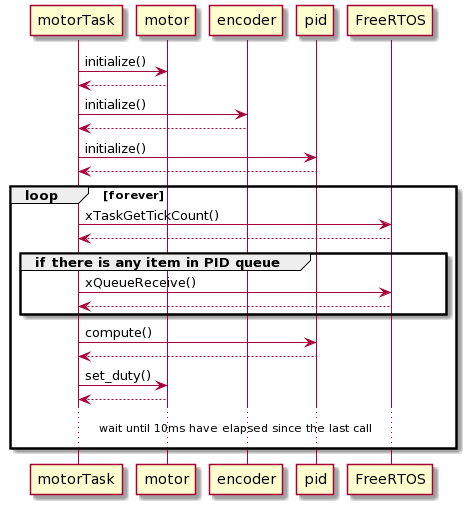
\includegraphics[width=0.5\textwidth]{img/motorTask_uml.png}
        \caption{Diagram aktywności procesu PID}
        \label{fig:pid_plantuml}
    \end{figure}